
\section{Kalibrierung}

\begin{frame}[b]
	\begin{figure}
		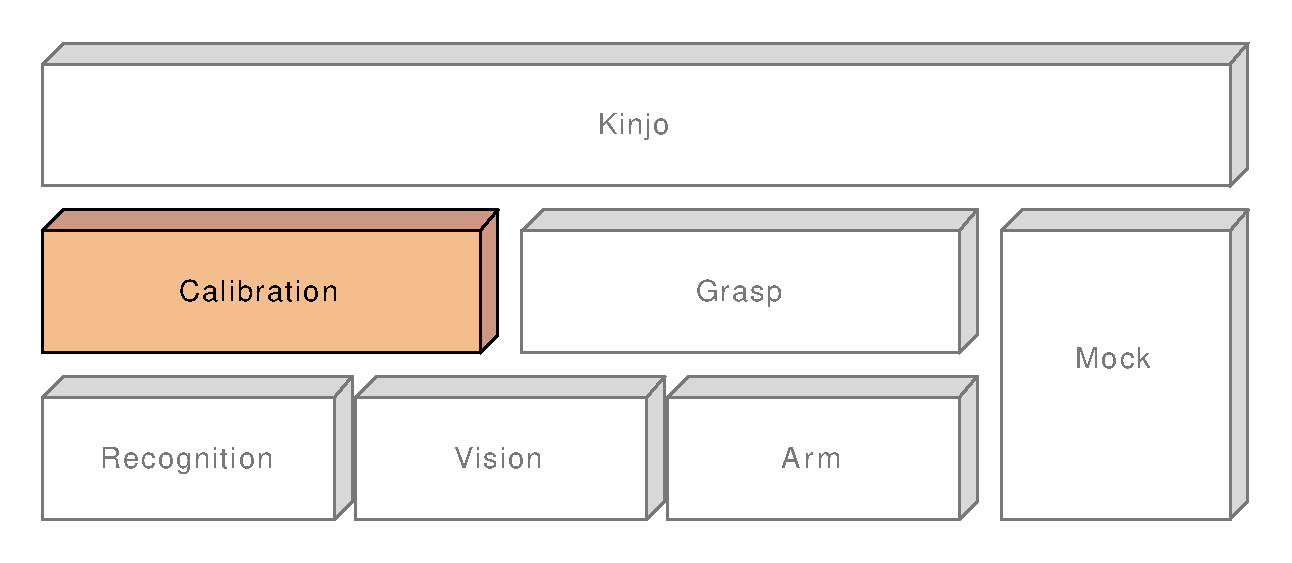
\includegraphics[width=0.8\textwidth]{nav_calibration}
	\end{figure}
	\vspace*{0.7cm}
\end{frame}

\begin{frame}[t]{Kinect}
	\begin{block}{Kalibrierung}
		\begin{itemize}
			\item Asynchron zur Hauptanwendung, damit Bildausgabe weiter läuft
			\item Fährt $P$ (zufällige) Punkte an
			\item Lässt an diesen Punkten die Hand in $R$ unterschiedliche
				Rotationen fahren
			\item Nimmt $K$ Bilder auf und versucht jeweils das
				Kalibrierungsobjekt zu erkennen
			\item Filtert aus den $R \cdot K$ Ergebnispunkten Ausreißer heraus
				und mittelt das Ergebnis
			\item Speichert die (maximal) $P$ Korrespondenzen von Arm-Position
				und erkannter Kinect-Position
			\item Berechnung der Starrkörpertransformation mittels
				\enquote{Least-Squares Rigid Motion Using SVD}
				\cite{sorkine2009lsrmusvd}
		\end{itemize}
	\end{block}
\end{frame}

